%Численное решение
\chapter{ВЫЧИСЛИТЕЛЬНЫЙ МЕТОД}
\section{Метод Рунге-Кутта 4-го порядка}

 В связи с тем, что точное решение имеет большую вычислительную сложность, то воспользуемся методом Рунге-Кутта 4-го порядка для решения системы ОДУ\cite{BahvalJidkovKobel1987}. Согласно методу приближенное значение в последующих точках вычисляется по итерационной формуле:

\begin{equation}
	y_{i+1} = y_i + \frac{h}{6} (k_1 + 2 k_2 + 2 k_3 + k_4)
\end{equation} 

Коэффициенты в общем виде находятся по формулам:

\begin{align}
	&k_1= f(x_i, y_i)\\
	&k_2=f(x_i + \frac{h}{2}, y_i + \frac{h}{2}k_1)\\
	&k_3=f(x_i + \frac{h}{2}, y_i + \frac{h}{2}k_2)\\
	&k_4 =  f(x_i + h, y_i + h k_3)\\
\end{align}, где $h$ - величина шага сетки по $x$.

Относительно задачи, рассматриваемой в данной работе аналогом $x$ является время $t$. А аналогом $y$ - вектор $q$, описывающий состояние системы  (\ref{eq:vector}). Тогда уравнение $\frac{d}{dt}q = f(t, q)$ принимает вид (\ref{eq:syst}). Начальные условия задачи Коши нам известны из постановки задачи. 
Легко можно заметить, что по сравнению с аналитическим решением, в методе Рунге-Кутта требуется произвести меньшее количество арифметических операций, что критично для данной задачи, потому что требуется проводить анализ большого количества возможных состояний системы, а это значит каждый раз симулировать процесс. А вкупе с тем что данный численный метод имеет порядок точности $O(h^4)$, то было решено использовать данный метод для получения приближенных значений состояний системы для каждого момента времени. На рисунке \ref{fig:anchi} продемонстрированы графики зависимости состояния системы от времени для параметров $k_1 = k_2 = k_3 = 1.5$ и $m_1 = m_2 = m_3 = 1$ со значением шага $h=0.01$с, что дает в итоге точность $O(h^4) = 10^{-8}$. На основе графиков и порядка точности можно сделать вывод, что данной точности интегрирования достаточно для решения поставленной задачи.

\begin{figure}[h]
    \begin{minipage}[h]{0.5\linewidth}
    \center{
        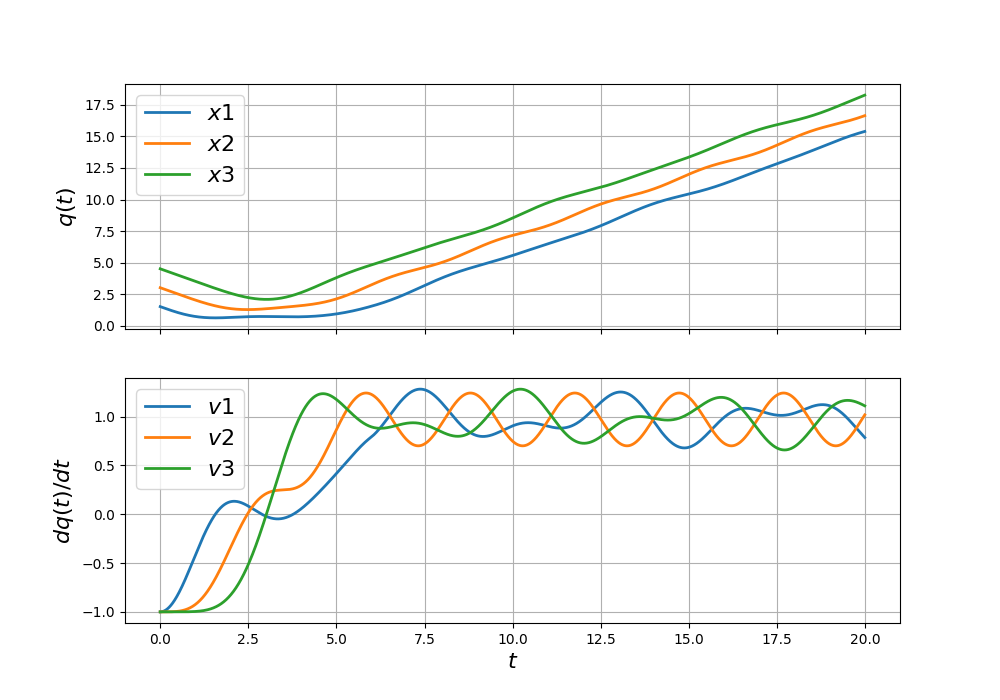
\includegraphics[width=1\textwidth]{analittraject.png} \\ a)
    }
    \end{minipage}
    \hfill  
    \begin{minipage}[h]{0.5\linewidth}
    \center{
         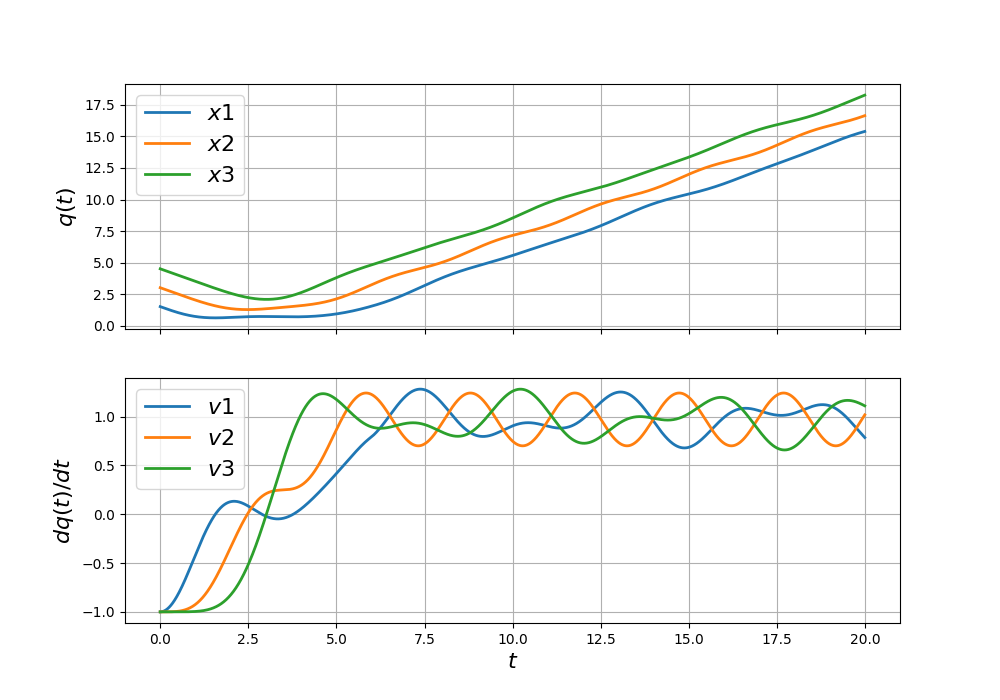
\includegraphics[width=1\textwidth]{rk4taject.png} \\ б)
    }
    \end{minipage}
    \caption{Траектории скоростей и координат системы трех тел, полученные аналитически (a) и численно (б) .}
    \label{fig:anchi}
\end{figure}